\begin{savequote}[75mm]
Science is a differential equation and religion is a boundary condition.
\qauthor{--- Alan Turing ---}
\end{savequote}

\chapter{Introduction}
\graphicspath{{figures/IntroDE/}}

%\begin{theorem} [Pythagorean theorem]
%\label{test}
%gfdgdg
%\end{theorem}
%
%\ref{test}
%
%
%\begin{example}
%\label{test}
%gfdgdg
%\end{example}
%
%
%
%
%\begin{mdframed}[backgroundcolor=gray!40,roundcorner=8pt]
%Input from question with output from my Mathematica version.
%Input is in input form, it can be copied and pasted to Mathematica.
%\begin{mmaCell}[functionlocal=y]{Code}
%  Integrate[{y^(-3)*(1-(a/y)^2)^(-2)},{y,r,Infinity}]
%\end{mmaCell}
%\begin{mmaCell}{Output}
%  \{ConditionalExpression[-\mmaFrac{1}{2 (\mmaSup{a}{2} - \mmaSup{r}{2})},
%     Im[r] Re[a] ≠ Im[a] Re[r] || ((a + r > 0 || a + r ∉ Reals) &&
%       ((Re[a] < r && Im[a] == 0) || a - r ∉ Reals)) || r ∉ Reals]\}
%\end{mmaCell}
%
%
%\end{mdframed}

\section{Mathematical modelling and simulation}
\label{models}
\subsection{Mathematical models}
In order to describe a biological, natural or physical process mathematically, we must  formulate it in mathematical terms; that is, we must construct a mathematical model\index{mathematical model} of the process. Once in place, it can be used to map one or more inputs related to the process at stake to one or multiple outputs as illustrated in Figure~\ref{Intro_1}. Below we give a more formal definition of a mathematical model. \index[aut]{Wiskundig model}

\begin{definition} [Mathematical model]
A \textbf{mathematical model} (\textit{wiskundig model}) is an abstract, simplified description of a part of reality that is created for a particular purpose. 
\end{definition}
\index{mathematical model}
\index[aut]{wiskundig model}

From this definition we infer several important aspects of mathematical models. Firstly, they are abstract because they are based on mathematical formalism, i.e.\ mathematical equations. Secondly, they constitute a simplified representation of the studied process(es), which implies that their development typically involves some simplifying assumptions, and hence that the modelling results only approximate the studied real-world processes up to some level. Thirdly, even though many other processes might affect the focal process, some of these are neglected, again possibly leading to discrepancies between the modelling results and the dynamics of real-world processes. Fourthly, and lastly, it is only meaningful to build a model if it is clear what question(s) it should be able to answer. A good mathematical model has two important properties:

\begin{itemize}
\item It is sufficiently simple so that the  problem can be solved.

\item It represents the actual situation sufficiently well so that the modelling results agree with observations to within a useful degree of accuracy. 
\end{itemize}

Clearly, if the modelling results do not agree with observations, the underlying assumptions of the model must be revised until satisfactory agreement is obtained. When sufficient agreement between the modelling results and observations is reached, i.e.\ the model got validated, it can be used to run simulations. 


\begin{definition} [Simulation]
\textbf{Simulation} (\textit{simulatie}) is the imitation of the operation of a real-world process by means of a mathematical model. 
\end{definition}
\index{simulation}
\index[aut]{simulatie}

Increasingly often such simulations are run on computers or computing clusters, and are therefore also referred to as \textit{in silico} experiments. 
\index{\textit{in silico} experiment}
\index[aut]{\textit{in silico} experiment}

\begin{figure}[h]
	\begin{center}
			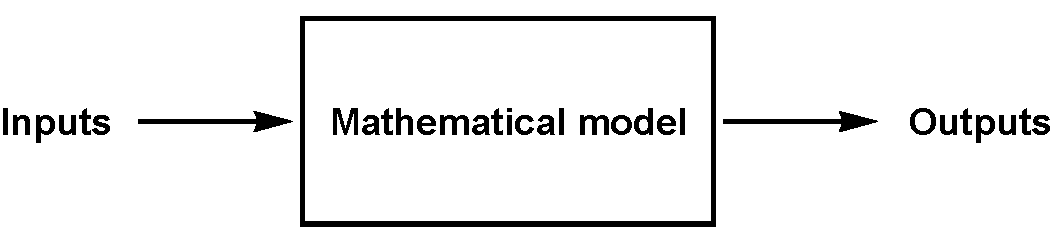
\includegraphics[width=0.5\textwidth]{Intro_1.pdf}
	\caption{Schematic representation of the functioning of a mathematical model. }
	\label{Intro_1}
	\end{center}
\end{figure}

In contrast to general thinking, everyone is nowadays on a daily basis often confronted with mathematical models or results obtained therewith. For instance, the weather forecast is based on dedicated weather models that describe atmospheric processes such as radiation, turbulence, evaporation, and so on. Indeed, for compiling its weather forecasts Belgium's Royal Meteorological Institute uses the weather model ALARO. Similarly, the Flemish Environment Agency (VMM) uses hydrological models to  forecast the water level in Flemish rivers, and, in the case of inundations, to forecast their extent and the water height above the ground level in real time \footnote{\url{https://www.waterinfo.be/}}.

\subsection{Model development}
Many physical problems concern relationships between changing quantities. Since rates of change are represented mathematically by
derivatives, mathematical models often involve equations relating an unknown function and one or more of its derivatives.

Consider for instance the rate of change of the velocity of a free-falling object with mass $m$ [M] in a vacuum, and suppose that we want to know the velocity  $v$ [L\,T$^{-1}$] of this object over time [T]; this the goal of our mathematical model. In that case, there is only one force exerted on this object, namely the gravitational force $m\,g$ [M\,L\,T$^{-2}$], where $g$ is the acceleration due to gravity. If we assume that the velocity $v$ of the object is positive in the downward direction, the velocity and gravitational vectors point in the same direction. So, we know from Newton's second law that
the instantaneous acceleration $a$ [L\,T$^{-2}$] of an object with constant mass $m$ is related to this force as:
\begin{equation}
m\,a=m\,g\,,
\end{equation}
or equivalently
\begin{equation}
a=g\,.
\label{freefall1}
\end{equation}
As the acceleration of an object $a$ is nothing but the rate of change of its velocity, we can rewrite Equation~\eqref{freefall1} using the derivative of $v(t)$ as:
\begin{equation}
\dfrac{d v}{d t}=g\,.
\label{freefall2}
\end{equation}
The solution of Equation~\eqref{freefall2} we are looking for is not just a scalar value like in the case of algebraic equations, but rather the function $v(t)$. Since this equation contains the derivative of this unknown function, it is referred to as a \textbf{differential equation} (\textit{differentiaalvergelijking}). 

The mathematical model based on Equation~\eqref{freefall2} has the initial velocity as input, while its output will be the velocity of the falling object over time. Its practical value, however, will be limited because it is based on the simplifying assumption that the object is falling in a vacuum. Fortunately it can be brought closer to reality by accounting for the drag force that acts on the object as it is moving downwards. This drag force acts in the direction opposite to the one of the gravitational force, and is often assumed to be proportional to the velocity of the falling object, so the more realistic counterpart of Equation~\eqref{freefall2} becomes
\begin{equation}
m\,\dfrac{d v}{d t}=m\,g-\mu\,v\,,
\label{freefall3}
\end{equation}
where $\mu$ [M\,T$^{-1}$] is the drag coefficient. Figure~\ref{FreeFall_1} shows different solutions of Equation~\eqref{freefall3} for $g=9.81$ \si{m.s^{-2}}, $m=75$ \si{kg}, $\mu=5.28$ \si{kg.s^{-1}}  and an initial velocity $v_0$ varying between $0$ and $240$ \si{m.s^{-1}}. It is clear that the initial velocity has only an impact on how fast the terminal velocity is reached, but not on the terminal velocity itself. 

\begin{figure}[h!]
	\begin{center}
			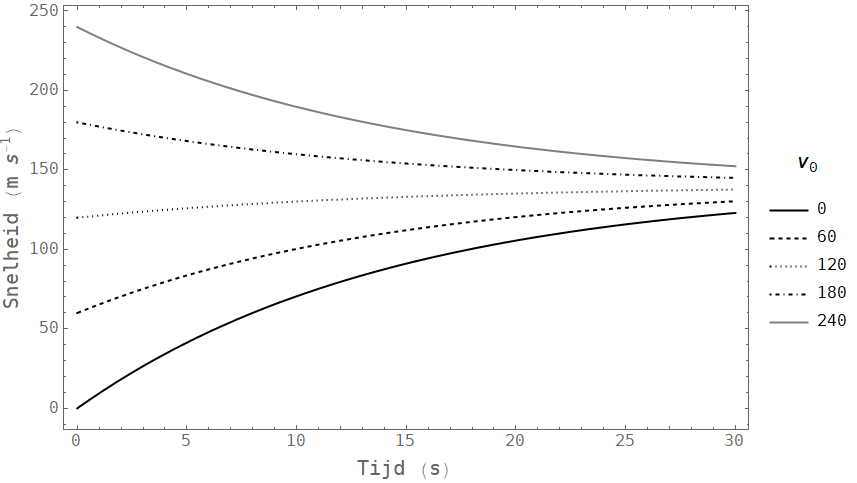
\includegraphics[width=0.6\textwidth]{FreeFall_1}
	\caption{Solutions of  Equation~\eqref{freefall3} for $g=9.81$ \si{m.s^{-2}}, $m=75$ \si{kg}, $\mu=5.28$ \si{kg.s^{-1}}  and initial velocity $v_0$ varying between $0$ and $240$ \si{m.s^{-1}}.}
	\label{FreeFall_1}
	\end{center}
\end{figure}

In addition to processes that involve a continuous change over time, there are also many processes that bring along a change only after a fixed amount of time has passed, such as reproductive events of many animals like fish (e.g.\ pike) and butterflies (e.g.\ the box moth). In these cases it becomes more meaningful to track, for instance, the species population size at discrete points in time, so we shall consider populations with a fixed time period between generations. Thus, we shall describe population size by a sequence ${N_k}$, with $N_0$ [--] denoting the initial population size, $N_1$ the population size of the first generation (at time step $1$), $N_2$ the population size of the second generation (at time step $2$), and so on. In the case of the box moth (\textit{Cydalima perspectalis}), the population changes only through eggs hatching and caterpillars entering the pupa stage, which happens at rates $e$ [--] and $p$ [--], respectively. Then, the size of the box moth population at a time step $k+1$ is given by
\begin{equation}
	N_{k+1}=\left(e-p\right)N_k\,,
\end{equation}
or upon introducing the net growth $r=e-p$ [--]:
\begin{equation}
	N_{k+1}=r\,N_k\,.
	\label{malthus}
\end{equation}
The mathematical model based on Equation~\eqref{malthus} is referred to as the model of Malthus, and the type of equation it uses is called a \textbf{difference equation} (\textit{differentievergelijking}).\index{difference equation}\index{Malthus model}\index[aut]{Model van Malthus} \index[aut]{differentievergelijking}
The long-term population size when starting from an initial population of size $N_0$ can be forecast by iteratively replacing $N_k$ by $r\,N_{k-1}$ in the right-hand side of Equation~\eqref{malthus}:
\begin{eqnarray*}
N_{k+1}&=&r\,N_k\\
&=&r^2\,N_{k-1}=r^3\,N_{k-2}\\
&=&r^{k+1}\,N_0\,.
\end{eqnarray*}
We infer that the population will grow exponentially if $r>1$ and evolve to 0 if $r<1$. In reality, the exponential growth dictated by this model is of course very unrealistic because the more individuals that are already present in a region and use its resources, the more difficult it will become to sustain yet another individual. Suppose the environment of a given region can support $K$ [--] individuals, i.e.\ the carrying capacity of the environment, then  Equation~\eqref{malthus} can be reformulated as
\begin{equation}
	N_{k+1}=r\left(1-\dfrac{N_k}{K}\right)N_k\,.
	\label{verhulst}
	\index{Verhulst model}
    \index[aut]{model van Verhulst}
\end{equation}
The mathematical model based on this equation is widely known as the model of Verhulst and is an example of a logistic population model. Figure~\ref{VerhulstFig} visualizes for different net growth rates the population size over time of a box moth population occupying an environment that can support up to 200 individuals ($K=200$) starting from an initial population with two individuals. As opposed to the impact of the drag coefficient $\mu$ on the terminal velocity (Figure~\ref{FreeFall_1}), the net growth rate $r$ does not only affect the road towards the terminal population, but also the terminal population size itself. Moreover, it seems that for some net growth rates (e.g.\ $r=3.5$) the population size does not converge to a constant value but keeps fluctuating. 

\begin{figure}
	\begin{center}
			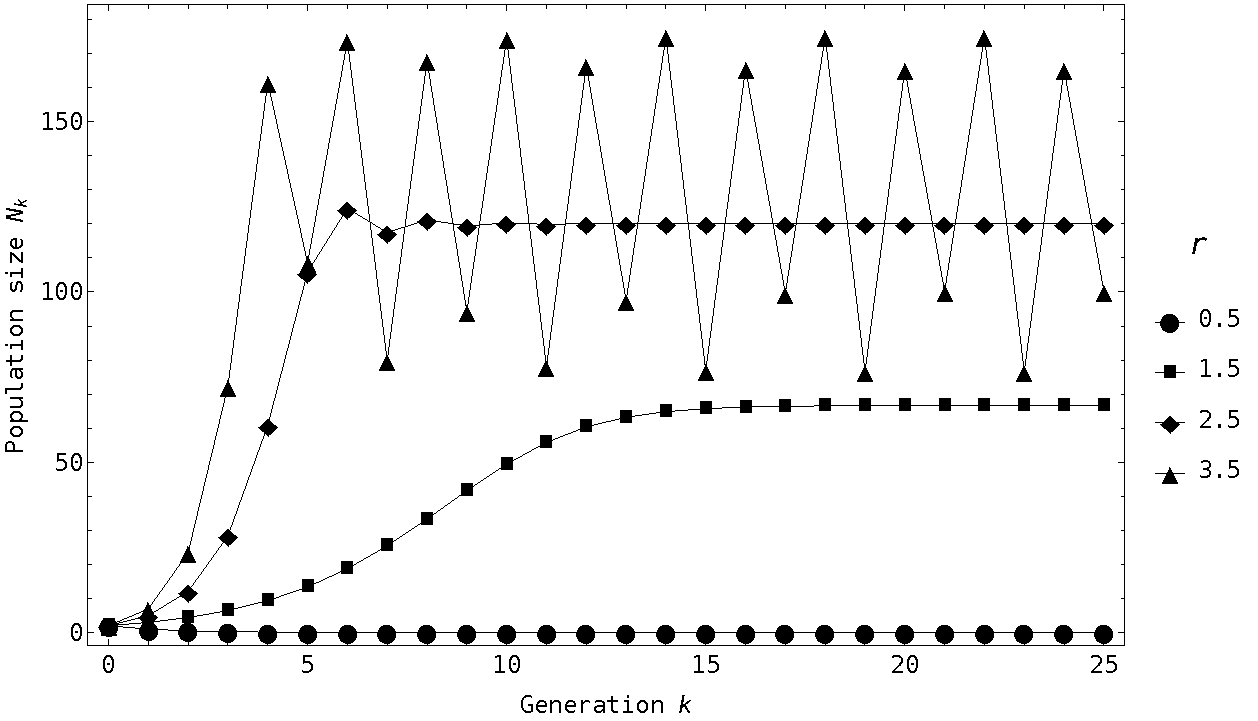
\includegraphics[width=0.6\textwidth]{Verhulst.pdf}
	\caption{Population size of a box moth population over time as given by Equation~\eqref{verhulst} for a carrying capacity $K=200$ and different net growth rates $r$.}
	\label{VerhulstFig}
	\end{center}
\end{figure}

From the two examples given in this section, it should be clear that mathematical models are very useful for gaining insights into  long-term behaviour, while they also allow to investigate what might happen in different scenarios. This is, however, possible only when one has good understanding of the equations underlying those models. 

\section{Differential and difference equations}
Here, we will introduce the formal definitions of both differential and difference equations, and also have a look at their established nomenclature. 
\subsection{Differential equations}
\label{naamgeving}
\subsubsection{Nomenclature}

\begin{definition} [Differential equation]
A  \textbf{differential equation} (\textit{differentiaalvergelijking}) is an equation that contains one or more derivatives of an unknown function $y=g(t)$, or mathematically, a differential equation is any equation that can be written as:
\begin{equation}
F\left(t,y,\dfrac{d y}{d t},\dfrac{d^2 y}{d t^2},\ldots,\dfrac{d^n y}{d t^n}\right)=0\,.
\label{DV_Def_1}
\end{equation}
\end{definition}
The \textbf{order} (\textit{orde}) of a differential equation corresponds to the order of the highest-order derivative that appears in the differential equation, while the \textbf{degree} (\textit{graad}) of a differential equation is the power to which the highest order derivative is raised. So, Equation~\eqref{DV_Def_1} may be referred to as an $n$-th order differential equation of degree one. Similarly, the differential equation we encountered in Section~\ref{models} for describing the velocity of a free-falling object (Equation~\eqref{freefall3}) was a first-order differential equation of degree one. 
\index{order}
\index[aut]{orde}
\index[aut]{graad}
\index{degree}
Equation~\eqref{DV_Def_1} gives the
implicit form of a differential equation. More commonly, we write differential equations in some explicit way, for instance, by isolating the highest order derivative:
$$
\dfrac{d^n y}{d t^n}=f\left(t,y,\dfrac{d y}{d t},\dfrac{d^2 y}{d t^2},\ldots,\dfrac{d^{n-1} y}{d t^{n-1}}\right)\,,
$$
or upon introducing the shorthand notation $y^{(n)}=\frac{d^n y}{d t^n}$:
\begin{equation}
y^{(n)}=f\left(t,y,y',y'',\ldots,y^{(n-1)}\right)\,.
\label{DV_Def_2}
\end{equation}
Alternatively, we might separate the unknown function and its derivatives from the terms that involve the independent variable only,
\begin{equation}
G\left(t,y,y',y'',\ldots,y^{(n)}\right)=q(t)\,, 
\label{DV_Def_3}
\end{equation}
where $G$ and $q$ are just functions. When the latter function $q(t)$ is identically zero, Equation~\eqref{DV_Def_3} is called a \textbf{homogeneous differential equation} (\textit{homogene differentiaalvergelijking}). Otherwise, it is a non-homogeneous differential equation, and $q(t)$ is referred to as the
\textbf{non-homogeneous term} (\textit{niet-homogene term}).
\index{homogeneous differential equation}
\index[aut]{homogene differentiaalvergelijking}
\index{non-homogeneous differential equation}
\index[aut]{inhomogene differentiaalvergelijking}

\begin{definition} [Linear differential equation]
\label{deflineair}
An $n$-th order differential equation is called \textbf{linear} (\textit{lineair}) if it is linear in the terms involving the unknown function and its derivatives, and hence can be written as
$$
F\left(t,y,y',y'',\ldots,y^{(n)}\right)=a_n(t)\,y^{(n)}+a_{n-1}(t)\,y^{(n-1)}+\cdots+a_2(t)\,y''+a_1(t)\,y'+a_0(t)\,y+b(t)=0\,.
$$
Otherwise, it is called \textbf{non-linear} (\textit{niet-lineair}).
\end{definition}
\index{linear differential equation}
\index[aut]{lineaire differentiaalvergelijking}

The differential equation we proposed in Section~\ref{models} to describe the velocity of a free-falling object (Equation~\eqref{freefall3}) was a linear first-order differential equation. In Chapters~\ref{First_Order_Quan}, \ref{Higher_Order} and \ref{First_Order_System_Quan} we will review the most important analytical and numerical solution methods for such differential equations and systems thereof. 

For many processes, the rate of change of the studied quantity depends only on the system, described by $y(t)$, and not on external factors. Describing such processes can be done using so-called autonomous differential equations. 
\begin{definition} [Autonomous differential equation]
A differential equation is called \textbf{autonomous} (\textit{autonoom}) if none of its terms depend explicitly on the independent variable $t$, so mathematically
$$
H\left(y,y',y'',\ldots,y^{(n)}\right)=0\,.
$$
\end{definition}
\index{autonomous differential equation}
\index[aut]{autonome differentiaalvergelijking}


A differential equation is an \textbf{ordinary differential equation} (\textit{gewone differentiaalvergelijking}) if it involves an unknown function of only one variable, or a \textbf{partial differential equation} (\textit{parti\"ele differentiaal vergelijking}) if it involves partial derivatives of a function of more than one variable. For instance, let $T(x,y)$ denote the temperature in some point $(x,y)$ of a room, then the partial differential equation that describes the temperature distribution of the room is given by
$$
\dfrac{\partial^2 T}{\partial x^2}+\dfrac{\partial^2 T}{\partial y^2}=0\,.
$$
\index{partial differential equation}
\index[aut]{parti\"ele differentiaalvergelijking}

In the remainder of this course, the focus will, however, be on ordinary differential equations, from now on referred to as differential equations for short. 



\subsubsection{Solutions of differential equations}

A solution of a differential equation is a function that satisfies the differential equation on some open $t$ interval;   thus, $y(t)$
is a solution of Equation~\eqref{DV_Def_2} if 1) $y(t)$ is $n$ times differentiable and 2)
$$
y^{(n)}(t)=f(t,y(t),y'(t), \dots,y^{(n-1)}(t))
$$
for all $t$ in some open interval $\left.\right]a,b\left[\right.$. From this we infer that it is in general not possible to define a priori the open interval $\left.\right]a,b\left[\right.$, though in the subsequent chapters we will see that this can be done for linear differential equations. 

The graph of a solution of a differential equation is called a
\textbf{solution curve} (\textit{oplossingsgrafiek}), so the curves in Figure~\ref{FreeFall_1} were nothing but solution curves of Equation~\eqref{freefall3} for different initial velocities. \index{solution}\index{solution curve}\index[aut]{oplossing}\index[aut]{oplossingscurve}


\begin{example}\label{example:1.2.1}
 Show that if $C_1$ and $C_2$ are constants then
\begin{equation} \label{eq:1.2.7}
y(t)=(C_1+C_2t)e^{-t}+2t-4
\end{equation}
 is a solution of the following linear second-order differential equation
\begin{equation} \label{eq:1.2.8}
y''+2y'+y=2t
\end{equation}
 on the open interval $\left.\right]-\infty,+\infty\left[\right.$.
\pagebreak

\xhrulefill{gray}{2.5pt}Solution \xhrulefill{gray}{2.5pt}

 Differentiating Equation~\eqref{eq:1.2.7} twice yields
$$
y'(t)=-\left(C_1+C_2t\right)e^{-t}+C_2e^{-t}+2
$$
 and
$$
y''(t)=\left(C_1+C_2t\right)e^{-t}-2C_2e^{-t}\,.
$$
Substituting these expressions into the left-hand side of Equation~\eqref{eq:1.2.8} one gets
$$
\left(C_1+C_2t\right)e^{-t}-2C_2e^{-t}+2\big[-\left(C_1+C_2t\right)e^{-t}+C_2e^{-t}+2\big]+\left(C_1+C_2t\right)e^{-t}+2t-4\,,
$$
and after some algebra:
$$
\left(1-2+1\right)\left(C_1+C_2t\right)e^{-t}+\left(-2+2\right)C_2e^{-t}+4+2t-4=2t\,,
$$
for all values of $t$.
Therefore $y(t)$ is a solution of Equation~\eqref{eq:1.2.8} on the open interval $\left.\right]-\infty,+\infty\left[\right.$.
\end{example}

In the next example, we will see that the open interval $\left.\right]a,b\left[\right.$ does not necessarily stretch from $-\infty$ to $+\infty$, and that there might be points where the solution is not defined. 

\begin{example}\label{example:1.2.2} 
Determine the open interval(s) $\left.\right]a,b\left[\right.$ where 
\begin{equation} \label{eq:1.2.5}
y(t)=\dfrac{t^2}{3}+\dfrac{1}{t}
\end{equation}
is a solution of
\begin{equation} \label{eq:1.2.6}
ty'+y=t^2\,.
\end{equation}

\xhrulefill{gray}{2.5pt}Solution \xhrulefill{gray}{2.5pt}

Substituting Equation~\eqref{eq:1.2.5} and its first-order derivative
$$
y'(t)=\dfrac{2t}{3} - \dfrac{1}{t^2}
$$
into the left-hand side of Equation~\eqref{eq:1.2.6} yields
$$
t \left(\dfrac{2t}{3} - \dfrac{1}{t^2}\right)+
\left(\dfrac{t^2}{3}+\dfrac{1}{t}\right)\,.
$$
This equals $t^2$ only if $t\ne0$. So, $y(t)$ is a solution of Equation~\eqref{eq:1.2.6} on $\left.\right]-\infty,0\left[\right.$ and $\left.\right]0,+\infty\left[\right.$.  However, $y(t)$ is not a solution of the differential equation on any open interval that contains $t=0$, since  $y(t)$ is not defined at  $t=0$.

Figure~\ref{Example2} shows the graph of Equation~\eqref{eq:1.2.5}. The part of the graph of Equation~\eqref{eq:1.2.5} on $\left.\right]0,+\infty\left[\right.$ is a solution curve of Equation~\eqref{eq:1.2.6}, as is the part of the graph on $\left.\right]-\infty,0\left[\right.$.

\begin{figure}[H]
	\begin{center}
			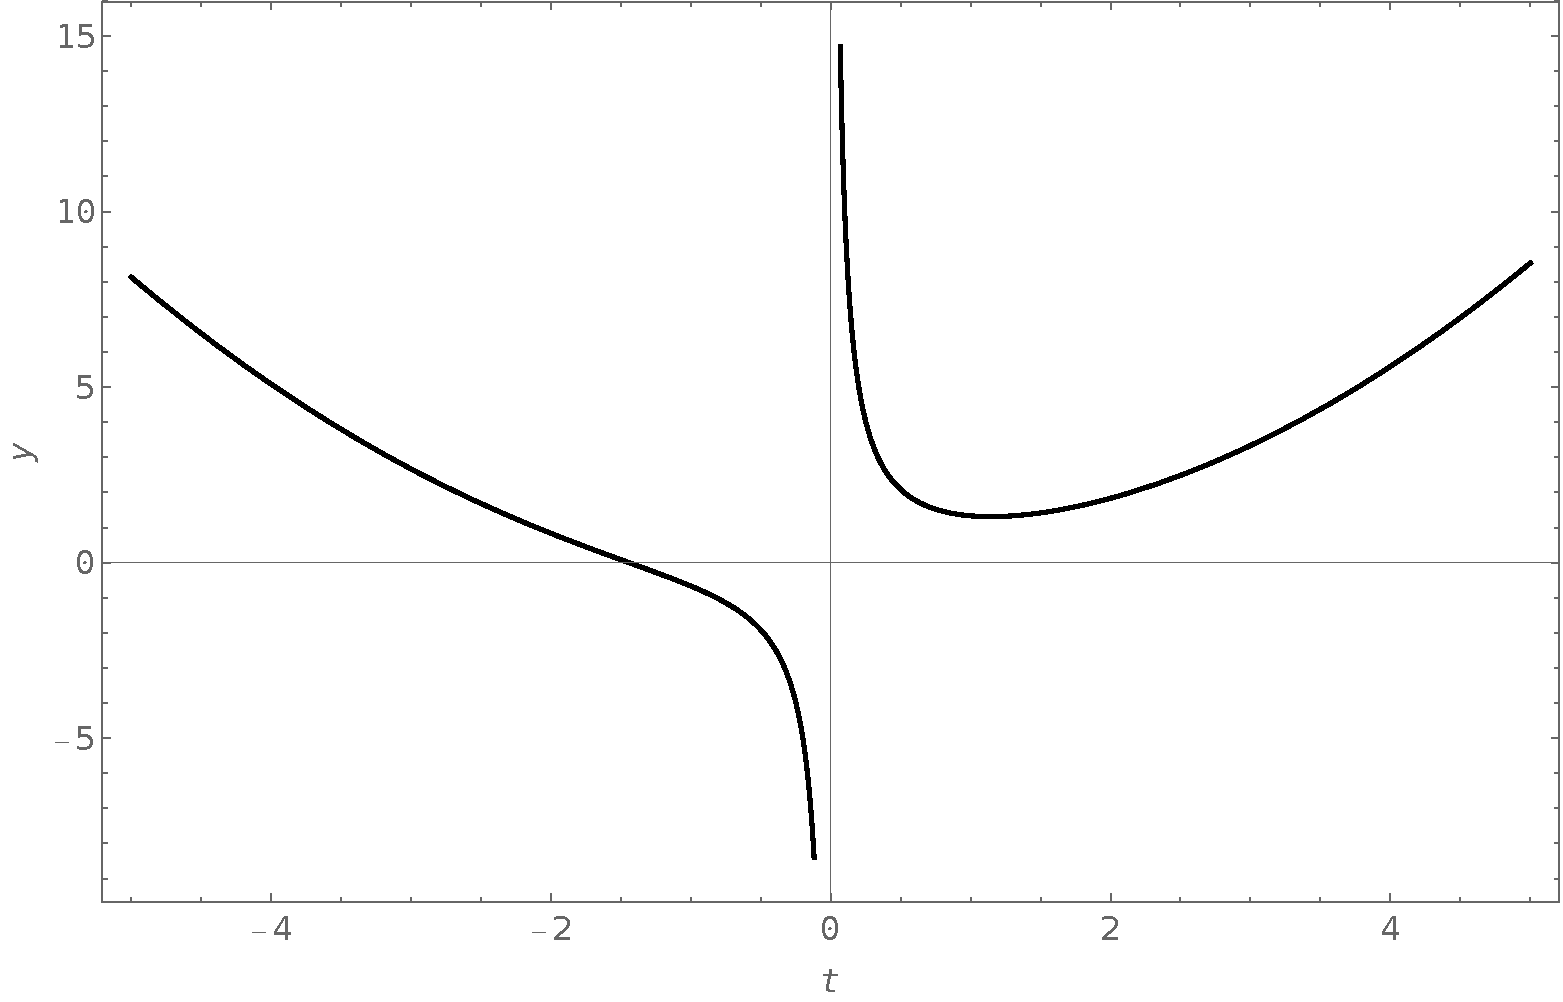
\includegraphics[width=0.6\textwidth]{Example_2.pdf}
	\caption{Solution curves of Equation~\eqref{eq:1.2.6}.}
	\label{Example2}
	\end{center}
\end{figure}

\end{example}



In Example~\ref{example:1.2.1} we saw that the differential equation $y''+2y'+y=2t$ has an infinite family of solutions that depend upon
2 arbitrary constants $C_1$ and  $C_2$. We refer to such a solution still involving constants as the \textbf{general solution} (\textit{algemene oplossing}) of a differential equation. \index{general solution}\index[aut]{algemene oplossing}In the absence of additional conditions, there is no reason to prefer one solution over another. However, often we will be interested in finding a solution of a differential equation that satisfies one or more specific conditions. Suppose, for instance, that we know the initial state of the system described by means of Equation~\eqref{eq:1.2.8}. More precisely, let us assume that $y(0)=1$ and $y'(0)=0$, i.e.\ we know one point on the solution curve of Equation~\eqref{eq:1.2.8} and one point on the curve describing the first-order derivative of $y(t)$. Plugging these two points in Equation~\eqref{eq:1.2.7} and its first-order derivative, respectively, we arrive at the following system of equations:
$$
\begin{array}{rcl}
1&=&C_1-4,\\
0&=&-C_1+C_2+2.
\end{array}
$$
From this we immediately see that $C_1=5$ and $C_2=3$, so that the solution of Equation~\eqref{eq:1.2.8} satisfying the imposed conditions becomes
$$
y(t)=(5+3t)e^{-t}+2t-4\,.
$$
The solution of Equation~\eqref{eq:1.2.8} we obtained by assigning particular values to the arbitrary constants in its general solution (Equation~\eqref{eq:1.2.7}) is referred to as a \textbf{particular solution} (\textit{particuliere oplossing}) of the differential equation. \index{particular solution}\index[aut]{particulier oplossing}

Problems that involve both a differential equation and information of the initial state of the studied system are of interest in many disciplines, and are referred to as initial value problems. A more formal definition is given below. 


\begin{definition} [Initial value problem]
\label{defivp}
An \textbf{initial value problem} (\textit{beginwaardeprobleem}) consists of an $n$-th order differential equation
$$
F\left(t,y,y',y'',\ldots,y^{(n)}\right)=0\,,
$$
defined for $t$ in an open interval $\left.\right]a,b\left[\right.$ and a set of $n$ initial conditions
$$
\begin{array}{rcl}
y(t_0)&=&y_0,\\
y'(t_0)&=&y_1,\\
y''(t_0)&=&y_2,\\
&\vdots&\\
y^{(n-1)}(t_0)&=&y_{n-1},\\
\end{array} 
$$
where $t_0$ lies in $\left.\right]a,b\left[\right.$, and $y_0$, $y_1$, \ldots, $y_{n-1}$ are given constants.
\end{definition}
\index{initial value problem}
\index[aut]{beginwaardeprobleem}
From this definition it is clear that we will need $n$ initial conditions in order to be able to solve an initial value problem involving an $n$-th order differential equation. Consistent with the definition of a solution of the $n$-th order differential equation given by Equation~\eqref{DV_Def_2}, we say that $y(t)$ is a solution
of the initial value problem stated in Definition~\ref{defivp} if 1) $y(t)$ is $n$ times
differentiable and 2)
$$
y^{(n)}(t)=f(t,y(t),y'(t), \dots,y^{(n-1)}(t))
$$
for all $t$ in some open interval $\left.\right]a,b\left[\right.$  that contains $t_0$, and 3) $y(t)$ satisfies the imposed initial conditions. In the remainder of this course, we will use the notation $y_{(t_0,y_0)}(t)$ to denote the solution of a differential equation that satisfies $y(t_0)=y_0$. 

The largest open interval that contains $t_0$ on which $y(t)$ is defined and satisfies the differential equation is called the \textbf{interval of existence} (\textit{bestaansinterval}). Let us now see what this all gives for Equation~\eqref{freefall3}. \index{interval of existence}\index[aut]{bestaansinterval}

\begin{example}\label{exFreefall} 
\ifmathematica
Determine with Mathematica the solution of\fi
\ifpython
Determine with Python the solution of\fi
$$
m\,\dfrac{d v}{d t}=m\,g-\mu\,v
$$
that satisfies the initial condition $v(0)=v_0$.

\xhrulefill{gray}{2.5pt}Solution \xhrulefill{gray}{2.5pt}

\ifmathematica
Let us first of all compute the general solution  of Equation~\eqref{freefall3}. In Mathematica, this is possible using the function \lstinline{DSolve} as follows: 
\begin{mdframed}[default,backgroundcolor=gray!40,roundcorner=8pt]
%\begin{mmaCell}{Input}
%	NDSolve[m \mmaSub{\(\pmb{\partial}\)}{t}v[t]==m \
%g-\mmaUnd{\(\pmb{\mu}\)} v[t],v[t],t]
%\end{mmaCell}
\begin{mmaCell}{Input}
  DSolve[m*D[v[t],t] == m*g-mu*v[t], v[t], t]
\end{mmaCell}

\begin{mmaCell}{Output}
	 \{\{v[t]\(\to\)\mmaFrac{g m}{mu}+\mmaSup{e}{-\mmaFrac{t mu}{m}} C[1]\}\}
\end{mmaCell}
\end{mdframed}
Note the double $=$ in the input line to express equality! Furthermore, note that curly brackets in Mathematica indicate a list, so our output is a list within a list. This is due to the fact that \lstinline{DSolve} can lead to multiple solutions. These are given as replacement rules (denoted by arrows) within a list, that are all again collected in one list.
Lastly, as can be inferred from the output, Mathematica uses C[1] to denote the arbitrary constant in the general solution. The particular solution satisfying $v(0)=0$ can also be computed easily in Mathematica by providing it with the appropriate initial condition:
\begin{mdframed}[default,backgroundcolor=gray!40,roundcorner=8pt]
%\begin{mmaCell}{Input}
%  sol=DSolve[\{m \mmaSub{\(\pmb{\partial}\)}{t}v[t]==m \
%g-\mmaUnd{\(\pmb{\mu}\)} v[t],v[0]==v0\},v[t],t]
%\end{mmaCell}
\begin{mmaCell}{Input}
  sol=DSolve[\{m*D[v[t],t] == m*g-mu*v[t], v[0] == v0\}, v[t], t]
\end{mmaCell}

\begin{mmaCell}{Output}
  \{\{v[t]\(\to\)\mmaFrac{\mmaSup{e}{-\mmaFrac{t mu}{m}} (-g \
m+\mmaSup{e}{\mmaFrac{t mu}{m}} g m+v0 mu)}{mu}\}\}
\end{mmaCell}
\end{mdframed}

Note that the particular solution was stored in the variable \lstinline{sol}. Upon choosing $v_0=0$ \si{m.s^{-1}}, $g=9.81$ \si{m.s^{-2}}, $m=75$ \si{kg} and $\mu=5.25$ \si{kg.s^{-1}}, we can plot the particular solution over the time interval $[0,30]$ using the Mathematica function \lstinline{Plot}. \index{\lstinline{Plot}}\index[aut]{\lstinline{Plot}}
For this, we can make use of the \lstinline{ReplaceAll} function, denoted for brevity by \lstinline{/.}, and the replacement rule of the previous output (\lstinline{sol}).
\begin{mdframed}[default,backgroundcolor=gray!40,roundcorner=8pt]
\begin{mmaCell}[moredefined={sol},morefunctionlocal={t}]{Input}
  v0=0;
		g=9.81;
		m=75;
		\mmaUnd{\(\pmb{\mu}\)}=5.25;
		Plot[v[t]/.\(\pmb{\,}\)sol,\{t,0,30\}]
\end{mmaCell}

\begin{mmaCell}[moregraphics={moreig={scale=.4}}]{Output}
	 \mmaGraphics{FreeFall_Math1.pdf}
\end{mmaCell}
\end{mdframed}

For the sake of clarity, it is even better to use a frame and add frame labels. Note that the arrows in the Mathematica syntax are obtained by typing \lstinline{->}.
\begin{mdframed}[default,backgroundcolor=gray!40,roundcorner=8pt]
\begin{mmaCell}[morefunctionlocal={t},moredefined={sol}]{Input}
  Plot[v[t]/.\(\pmb{\,}\)sol,\{t,0,30\},Frame\(\pmb{\to}\)True,FrameLabel\(\pmb{\to}\)\{"Time (s)","Velocity (m/s)"\}]
\end{mmaCell}

\begin{mmaCell}[moregraphics={moreig={scale=.4}}]{Output}
	 \mmaGraphics{FreeFall_Math2.pdf}
\end{mmaCell}
\end{mdframed}
\fi

\ifpython
Let us first of all compute the general solution  of Equation~\eqref{freefall3}. In Python, this is possible using the function \lstinline{dsolve} as follows: 
\begin{pyin}
from sympy import symbols, Function, Derivative, dsolve
t, g, m, mu = symbols('t g m mu')
v = Function('v')
v1 = Derivative(v(t), t)
dsolve(m*v1 - m*g + mu*v(t), v(t))
\end{pyin}
\begin{pyout}
v(t) = \frac{gm + e^{\frac{\mu(C_1 - t)}{m}}}{\mu}
\end{pyout}
As can be inferred from the output, Python uses $C_1$ to denote the arbitrary constant in the general solution. The particular solution satisfying $v(0)=0$ can also be computed easily in Python by providing it with the appropriate initial condition:
\begin{pyin}
from sympy import symbols, Function, Derivative, dsolve
t, g, m, mu = symbols('t g m mu')
v = Function('v')
v1 = Derivative(v(t), t)
sol = dsolve(m*v1 - m*g + mu*v(t), v(t), ics={v(0):v0})
sol
\end{pyin}
\begin{pyout}
v(t) = \frac{gm + e^{\frac{mu \left(\frac{m \log(-gm+\mu v0)}{\mu}-t\right)}{m}}}{\mu}
\end{pyout}

Note that the particular solution was stored in the variable \lstinline{sol}. Upon choosing $v_0=0$ \si{m.s^{-1}}, $g=9.81$ \si{m.s^{-2}}, $m=75$ \si{kg} and $\mu=5.25$ \si{kg.s^{-1}}, we can plot the particular solution over the time interval $[0,30]$ using the Python function \lstinline{plot}. \index{\lstinline{plot}}\index[aut]{\lstinline{plot}}
For this, we can make use of the \lstinline{subs} function and the replacement rule of the previous output (\lstinline{sol}).
\begin{pyin}
sol = sol.subs({m:75, g:9.81, mu:5.25, v0:0})
plot(sol.rhs, (t, 0, 30), (v, 0, 120), xlim=(0, 30), ylim=(0,120))
\end{pyin}
\begin{pyout}
|\includegraphics{figures/IntroDE/FreeFall_Math2_Python.pdf}|
\end{pyout}
\fi
\end{example}
So far, we only encountered differential equations whose solution can be written explicitly as a function of the independent variable $t$. In many cases, however, and especially when dealing with non-linear differential equations, we can only obtain an \textbf{implicit solution} (\textit{impliciete oplossing}) $S(t,y)=0$. Consider, for instance, the following  non-linear first-order differential equation, which does not look complicated at all. \index{implicit solution}\index[aut]{impliciete oplossing} \index{explicit solution}\index[aut]{expliciete oplossing}


\begin{example}
\ifmathematica
Determine and plot the solution of the differential equation
$$
y\,y' - y + t = 0\,. 
$$
that satisfies $y(1)=1$ using Mathematica.\fi

\ifpython
Determine and plot the solution of the differential equation
$$
y\,y' - y + t = 0\,. 
$$
that satisfies $y(1)=1$ using Python.
\fi

\pagebreak
\xhrulefill{gray}{2.5pt}Solution \xhrulefill{gray}{2.5pt}

\ifmathematica
The appropriate syntax for determining the general solution of this differential equation is: 
\begin{mdframed}[default,backgroundcolor=gray!40,roundcorner=8pt]
\begin{mmaCell}{Input}
  sol2 = DSolve[\{y[t]*D[y[t],t]-y[t]+t==0,y[1]==1\},y[t],t]
\end{mmaCell}
\end{mdframed}

Somehow surprisingly in the light of the simplicity of this differential equation, Mathematica returns only an implicit solution. 

\begin{mdframed}[default,backgroundcolor=gray!40,roundcorner=8pt]
\begin{mmaCell}{Output}
  Solve[\mmaFrac{ArcTan[\mmaFrac{-1+\mmaFrac{2y[t]}{t}}{\mmaSqrt{3}}]}{\mmaSqrt{3}}+\mmaFrac{1}{2}Log[1-\mmaFrac{y[t]}{t}+\mmaFrac{\mmaSup{y[t]}{2}}{\mmaSup{t}{2}}]==\mmaFrac{\(\pi\)}{6\mmaSqrt{3}}-Log[t],y[t]]
\end{mmaCell}
\end{mdframed}

Such an implicit solution can be visualized using the Mathematica function \lstinline{ContourPlot}. For this, we first have to extract the implicit function from the obtained solution, using the Mathematica function \lstinline{First}, and replace the \lstinline{y[t]} in the implicit solution by a variable. Then we simply copy and paste the result into \lstinline{ContourPlot}. \index{\lstinline{ContourPlot}} \index[aut]{\lstinline{ContourPlot}}
\begin{mdframed}[default,backgroundcolor=gray!40,roundcorner=8pt]

\begin{mmaCell}[moredefined={sol2}]{Input}
  First[sol2]/.\(\pmb{\,}\)\{y[t]\(\pmb{\to}\)y\}
\end{mmaCell}

\begin{mmaCell}{Output}
  \mmaFrac{ArcTan[\mmaFrac{-1+\mmaFrac{2y}{t}}{\mmaSqrt{3}}]}{\mmaSqrt{3}}+\mmaFrac{1}{2}Log[1-\mmaFrac{y}{t}+\mmaFrac{\mmaSup{y}{2}}{\mmaSup{t}{2}}]==\mmaFrac{\mmaDef{\(\pmb{\pi}\)}}{6\mmaSqrt{3}}-Log[t]
\end{mmaCell}

\begin{mmaCell}[morefunctionlocal={y, t}]{Input}
  ContourPlot[\mmaFrac{ArcTan[\mmaFrac{-1+\mmaFrac{2y}{t}}{\mmaSqrt{3}}]}{\mmaSqrt{3}}+\mmaFrac{1}{2}Log[1-\mmaFrac{y}{t}+\mmaFrac{\mmaSup{y}{2}}{\mmaSup{t}{2}}]==\mmaFrac{\mmaDef{\(\pmb{\pi}\)}}{6\mmaSqrt{3}}-Log[t],

	 \{t,0,3\},\{y,-4,4\},FrameLabel\(\pmb{\to}\)\{"t","y"\}]
\end{mmaCell}

\begin{mmaCell}[moregraphics={moreig={scale=.4}}]{Output}
	 \mmaGraphics{Impliciet_Vb.pdf}
\end{mmaCell}
\end{mdframed}
\fi

\ifpython
The appropriate syntax for determining the general solution of this differential equation is: 
\begin{pyin}
from sympy import symbols, Function, Derivative, dsolve
t = symbols('t')
y = Function('y')
y1 = Derivative(y(t), t)
dsolve(y(t)*y1 - y(t) + t, y(t), ics = {y(1):1})
\end{pyin}
Somehow surprisingly in the light of the simplicity of this differential equation, Python returns only an implicit solution. 
\begin{pyout}
\log(t) = -\log\left(\sqrt{1-\frac{y(t)}{t}+\frac{y^2(t)}{t^2}}\right) + \frac{\sqrt{3}\arctan\left(\frac{\sqrt{3}(1-\frac{2y(t)}{t})}{3}\right)}{3} + \frac{\sqrt{3}\pi}{18}
\end{pyout}
Such an implicit solution can be visualized using the Python function \lstinline{contour}.
\begin{pyin}
fig = plt.figure(figsize=(6,4))
ax = fig.add_axes([0,0,1,1])
ax.set_xlim(0, 3)
ax.set_ylim(-4, 4)

x = np.linspace(0, 2, 50)
y = np.linspace(-4, 1, 40)

x, y = np.meshgrid(x, y)

ax.contour(x, y, np.arctan((-1+2*y/x)/np.sqrt(3))/np.sqrt(3) + 1/2 * np.log(1-y/x+y**2/x**2) - np.pi/(6*np.sqrt(3)) + np.log(x), [0], colors='blue')

ax.set_xlabel('t')
ax.set_ylabel('y')
plt.show()
\end{pyin}
\begin{pyout}
|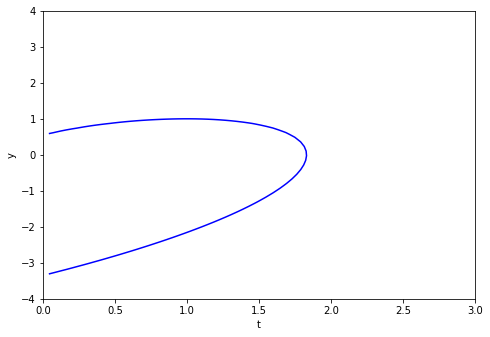
\includegraphics[width=0.5\textwidth]{figures/IntroDE/Impliciet_Vb_Python.png}|
\end{pyout}
\fi
\end{example}


\subsection{Difference equations}
\label{differenceEquations}
Though difference equations are not the main focus of this course, they are closely related to differential equations, with the main difference being that the independent variable is discrete. Hence, they can be viewed either as a discrete analogue of differential equations. Much of the terminology that was introduced for differential equations can also be used for difference equations, but let us first of all state a formal definition.

\begin{definition} [Difference equation]
A  \textbf{difference equation} (\textit{differentievergelijking}) is an equation that contains unknown quantities $y_i$, $i=0,1,\ldots,$
\begin{equation}
y_{n+k}=\mathcal{F}\left(y_{n+k-1},y_{n+k-2},\ldots,y_{n}\right)\,,
\label{DV_Dif_1}
\end{equation}
where $\mathcal{F}$ is some function and $k$ is the order of the difference equation. 
\end{definition}
Essentially, a difference equation recursively defines a sequence of values $y_i$, $i=0,1,\ldots$, once one or more initial terms are given: each further term of the sequence is defined as a function of the preceding terms. Hence, a difference equation is also sometimes referred to as a \textbf{recurrence relation} (\textit{recursiebetrekking}). \index{recurence relation}\index[aut]{recursiebetrekking}



Just as with differential equations, we can also define linear difference equations. 
\begin{definition} [Linear difference equation]
An $k$-th order difference equation is called \textbf{linear} (\textit{lineair}) if it can be written as
\begin{equation}
\mathcal{F}\left(y_{n+k-1},y_{n+k-2},\ldots,y_{n}\right)=a_k\,y_{n+k}+a_{k-1}\,y_{n+k-1}+\cdots+a_1\,y_{n+1}+a_0\,y_n+b=0\,.
\index{linear difference equation} \index[aut]{lineaire differentievergelijking}
\label{DV_Dif_2}
\end{equation}
Otherwise, it is called \textbf{non-linear} (\textit{niet-lineair}). 
\end{definition}
A linear difference equation like Equation~\eqref{DV_Dif_2} is \textbf{homogeneous} (\textit{homogeen}) if $b=0$. Otherwise, it is a \textbf{non-homogeneous} (\textit{niet-homogeen}) difference equation. The Malthus model that describes exponential growth and is based on Equation~\eqref{malthus} is an example of a linear first-order difference equation, whereas the more realistic Verhulst model is based on a non-linear first-order difference equation (Equation~\eqref{verhulst}). \index{homogeneous linear difference equation} \index[aut]{homogene lineaire differentievergelijking} \index{non-homogeneous linear difference equation} \index[aut]{niet-homogene lineaire differentievergelijking}

Again similar to the terminology used in the framework of differential equations, one either arrives at the \textbf{general solution} (\textit{algemene oplossing}) of the difference equation at stake, or one obtains a \textbf{particular solution} (\textit{particuliere oplossing}) that satisfies some additional conditions. In general, $k$ such conditions need to be specified in order to be able to find a particular solution of an $k$-th order difference equation.\index{general solution} \index[aut]{algemene oplossing}\index{particular solution} \index[aut]{particuliere oplossing}

\begin{example}
\ifmathematica
Let us try to find a general solution of Equation~\eqref{malthus}, i.e.
$$
N_{k+1}=r\,N_k
$$
using Mathematica.

In Mathematica, the function \lstinline{RSolve} solves difference equations. However, since \lstinline{N} is a built-in function of Mathematica, we replace $N$ by $y$ when implementing the difference equation, so:\index{\lstinline{RSolve}}\index[aut]{\lstinline{RSolve}}
\begin{mdframed}[default,backgroundcolor=gray!40,roundcorner=8pt]
\begin{mmaCell}{Input}
  RSolve[\{y[k+1]==r*y[k]\},y[k],k]
\end{mmaCell}

\begin{mmaCell}{Output}
  \{\{y[k]\(\to\)\mmaSup{r}{-1+k} C[1]\}\}
\end{mmaCell}
\end{mdframed}
Or, supposing that the initial population size is given by $N_0$:
\begin{mdframed}[default,backgroundcolor=gray!40,roundcorner=8pt]
\begin{mmaCell}{Input}
  sol3=RSolve[\{y[k+1]==r*y[k],y[0]==y0\},y[k],k]
\end{mmaCell}


\begin{mmaCell}{Output}
  \{\{y[k]\(\to\)\mmaSup{r}{k} y0\}\}
\end{mmaCell}
\end{mdframed}
So, we get
$$
N_k=r^k\,N_0\,,
$$
which agrees with what we inferred intuitively in Section~\ref{models}. Finally, using this solution we can easily plot the population size up to generation 15. For that purpose, we first use the Mathematica function \lstinline{Table} to generate a list containing the population sizes of the 15 first generations and then the function \lstinline{ListPlot}, which is suited to plot discrete data points. Note that, in order to make \lstinline{Table} work properly, we have to extract the replacement rule from the solution list, again using \lstinline{First}.
\index{\lstinline{ListPlot}}\index[aut]{\lstinline{ListPlot}}

\begin{mdframed}[default,backgroundcolor=gray!40,roundcorner=8pt]
\begin{mmaCell}[moredefined={sol2,Filling},morefunctionlocal={k}]{Input}
  r=1.5;
	 y0=2;
	 ListPlot[Table[y[k]/.\(\pmb{\,}\)First[sol2],\{k,1,15\}],\
Filling\(\pmb{\to}\)Axis,Frame\(\pmb{\to}\)True,

	 FrameLabel\(\pmb{\to}\)\{"Generation k","Population size \mmaSub{N}{k}"\}]
\end{mmaCell}
\begin{mmaCell}[moregraphics={moreig={scale=.4}}]{Output}
	 \mmaGraphics{Malthus_Vb.pdf}
\end{mmaCell}
\end{mdframed}
\fi

\ifpython
Let us try to find a general solution of Equation~\eqref{malthus}, i.e.
$$
N_{k+1}=r\,N_k
$$
using Python.

In Python, the function \lstinline{rsolve} solves difference equations.
\begin{pyin}
from sympy import Function, rsolve, symbols
r, k = symbols('r k')
N = Function("N")
f = N(k+1) - r*N(k)
sol = rsolve(f, N(k));
sol
\end{pyin}
\begin{pyout}
C_0 r^k
\end{pyout}
Or, supposing that the initial population size is given by $N_0$:
\begin{pyin}
from sympy import Function, rsolve, symbols
r, k, N0 = symbols('r k N0')
N = Function("N")
f = N(k+1) - r*N(k)
sol = rsolve(f, N(k), {N(0):N0});
sol
\end{pyin}
\begin{pyout}
N0 r^k
\end{pyout}
So, we get
$$
N_k=r^k\,N_0\,,
$$
which agrees with what we inferred intuitively in Section~\ref{models}. Finally, using this solution we can easily plot the population size up to generation 15. For that purpose, we first use the Python function \lstinline{lambdify} to generate a function from our solution. Then we use \lstinline{scatter} to plot the population size
\begin{pyin}
from sympy import Function, rsolve, symbols, lambdify
import numpy as np
import matplotlib.pyplot as plt

fig = plt.figure(figsize=(6,4))
ax = fig.add_axes([0,0,1,1])
ax.set_xlim(0, 15)
ax.set_ylim(0, 900)

k = symbols('k')
N = Function("N")
f = N(k+1) - 1.5*N(k)
sol = rsolve(f, N(k), {N(0):2})
lam = lambdify(k, sol)
for i in range(0, 16):
    ax.scatter([i], [lam(i)], color='black')
    ax.plot([i, i], [0, lam(i)], color='black')

ax.set_xlabel('Generation k')
ax.set_ylabel('Population size N$_k$')
plt.show()
\end{pyin}
\begin{pyout}
|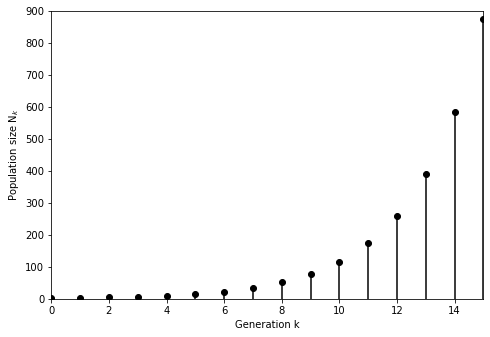
\includegraphics[width=0.5\textwidth]{Malthus_Vb_Python.png}|
\end{pyout}
\fi
\end{example}

\newpage
\section{Exercises}
\renewcommand{\ExerciseListName}{Assignement}
%oefening 2.1
\begin{Exercise} Determine the order and degree of the following differential equations..
	\begin{multicols}{2}
			\Question $dy + \left(ty-\cos(t)\right)\, dt=0$
			\Question $\left(y'''\right)^2+ty''+2y\left(y'\right)^3+ty=0$
			\Question $y''\,y'+t\,y'^3+y=0$ 
			\Question $y'+t=\left(y-ty'\right)^{-3}$
			\EndCurrentQuestion
	\end{multicols}

\end{Exercise}


\setboolean{firstanswerofthechapter}{true}
\begin{Answer}\phantom{} 
By rewriting the differential equations, we conclude:
    \begin{multicols}{2}
	    \Question first order, first degree
	    \Question third order, second degree
	    \Question second order, first degree
	    \Question first order, fourth degree
    \EndCurrentQuestion
    \end{multicols}
\end{Answer}
\setboolean{firstanswerofthechapter}{false}


%oefening 2.2
\begin{Exercise} Show that following families of curves can be written with one constant.
			\Question $y=C_1\, e^{t+C_2}$
			\Question $y=C_1+\ln |C_2 t|$
			\EndCurrentQuestion
\end{Exercise}

\begin{Answer}\phantom{} The families of curves can be rewritten as follows:
	    \Question $y = C_3e^{t}$ with $C_3 = C_1e^{C_2}$
	    \Question $y = C_3 + \ln |t|$ with $C_3 = C_1+\ln |C_2|$
    \EndCurrentQuestion
\end{Answer}

%oefening 2.3
\begin{Exercise} Show that the function $y(t)$ is a solution of the given differential equation. Then find the particular solution based on the initial conditions.
			\par
			\begin{flushright}
            \setlength{\arraycolsep}{0.28cm} 
            $\begin{array}{r|l|l|l}
            &\mbox{Differentiaalvergelijking} & \mbox{Oplossing} & \mbox{Beginvoorwaarde(n)}\\ 
            \hline
            \hline
            &&&\vspace{-0.3cm}\\
            \hspace{-0.2cm}\mbox{(a)} &  y + y' = t^3 + 3 t^2\quad\; & y(t) = t^3 + Ce^{-t} &  y(0)=3 \\
            \hspace{-0.2cm}\mbox{(b)} &  t y' - y = t^2 e^t & y(t) = Ct + t e^{t} &  y(1)=e \\
            %\hspace{-0.2cm}\mbox{(c)} &  2 y - 3 t + t y'= 0 & y(t) = t + \dfrac{C}{t^2} &  y(-3)=-2 \\
            \hspace{-0.2cm}\mbox{(c)} &  y - t y' - y'{^2} = 0 & y(t) = C t + C^2 &  y(2)=-1 \\
            %\hspace{-0.2cm}\mbox{(e)} &  2 y - 2 t y' + t^2 y'' = 0 & y(t) = C_1 t + C_2 t^2 &  y(1)=0; y'(1)=5 \\
            \hspace{-0.2cm}\mbox{(d)} &  y''' + y'' = 0 & y(t) = C_1 e^{-t} + C_2 t + C_3\quad\; &  y(0)=2,\, y'(0)= 1,\, y''(0)= 3\\
            %\hspace{-0.2cm}\mbox{(g)} &  ty' + y = t\sin t & y(t) = \dfrac{\sin t+C}{t}-\cos t  &  y(\pi)=1 \\
            \hspace{-0.2cm}\mbox{(e)} &  y' - y = 2(1-t) & y(t) = 2t+Ce^t  &  y(0)=3 \\ %ADB
            %\hspace{-0.2cm}\mbox{(f)} &   y'' -3 y'+2y=2t-3 = 0 & y(t) = C_1 e^{t} + C_2 e^{2t} + t &  y(0)=0; y'(0)=2 \\ %ADB
            %\hspace{-0.2cm}\mbox{(g)} &  y'' + y = 0 & y(t) = C_1 \cos t + C_2 \sin t  &  y(0)=0; y'(0)=1 %ADB
            \end{array}$
            \end{flushright}
			\EndCurrentQuestion
\end{Exercise}

\begin{Answer}\phantom{}  To show that $y(t)$ is a solution of the given differential equation, it suffices to differentiate $y(t)$, put it in the differential equation, and note that this yields zero.
To determine the particular solution on the basis of the initial conditions, it suffices to insert it into the differential equation.
	    \Question  $y(t) = t^3 + 3e^{-t}$
	    \Question $y(t) = te^t$
	    \Question $y(t) = 1 - t$
	    \Question $y(t) = 3e^{-t} + 4t - 1$
	    \Question $y(t) = 2t + 3e^t$
    \EndCurrentQuestion
\end{Answer}

%oefening 2.4
\begin{Exercise}Write the differential equations that describe the problems below.
            \Question 
            It has been empirically established that the rate at which the stomach contents of a predatory fish decreases is directly proportional to the square root of this volume.
            \Question During a chemical reaction, substance $A$ is converted to substance $B$ at a rate that is directly proportional to the square of the amount of substance $A$. Call $A(t)$ the amount of unreacted substance $A$ at time $t$.
            \Question Newton's law of cooling states that the temperature change of an object is directly proportional to the difference between the (variable) temperature $T(t)$ of the object itself and the (constant) temperature $R$ of the environment.
            \Question When a patient is infused with a constant amount of painkiller per hour, the body breaks down this drug at a rate that is directly proportional to the amount present. We call that amount $M(t)$, the constant supply $a$ and the degradation rate $v$ (with $0< v < 1$), the relative amount of degraded substance per unit time.
            \EndCurrentQuestion
\end{Exercise}

\begin{Answer}\phantom{} The differential equations describing the problems are given by:
 	   \Question $V'(t) = k\sqrt{V(t)}$,
	   \Question $A'(t) = k\,A(t)^2$,
	   \Question $T'(t) = k\left(T(t) - R\right)$,
	   \Question $M'(t) = a - v\,M(t)$.
	   \EndCurrentQuestion
\end{Answer}

%oefening 2.5
\begin{Exercise} Find and plot the solution of the following differential equations using
 \ifmathematica Mathematica.\fi \ifpython Python.\fi
    \Question $y'=1+2ty$,\qquad if \quad $y(2)=-1$ %BDB
    \Question $y'+2ty=4t$,\qquad if\quad $y(0)=5$ %BDB
    \Question $(2+\sin (y))y'+t=0$,\qquad if\quad $y(2)=0$ %BDB
    \Question $x^2\,y\,y'-e^y=0$,\qquad if\quad $y\left(1\right)=0$ %BDB-P1
    \Question $y'' + 2y'+5y=0$,\qquad if\quad $y(0)=2$\quad and \quad $y'(0)=2$ %BDB
    \Question $ty'' + \left(\cos(t)\right)y'+t^2y=t$,\qquad if\quad $y(-1)=-1$\quad and\quad $y'(-1)=2$ %BDB
    \Question $y^{(4)}-4y'''-5y''+36y'-36\,y=0$,\qquad if\quad $y(0)=1,~y'(0)=2,~y''(0)=3$ and $y'''(0)=4$ %BDB-P1
    \EndCurrentQuestion
\end{Exercise}

\begin{Answer}\phantom{}  We only give the instructions for e).
	    \Question $y'' + 2y'+ 5y = 0$, \qquad if \quad $y(0) = 2$ \quad en \quad $y'(0) = 2$.\\
	   
	   Determine solution with mathematica:\\
\begin{mdframed}[default,backgroundcolor=gray!40,roundcorner=8pt]
\begin{mmaCell}{Input}
  opl = DSolve[\{y''[t] + 2*y'[t] + 5*y[t] == 0, y[0] == 2, y'[0] == 2\}, 
  y[t], t]
\end{mmaCell}

\begin{mmaCell}{Output}
	 \{\{v[t]\(\to\) 2\mmaSup{e}{-t}(Cos[2t] + Sin[2t])\}\}
\end{mmaCell}
\end{mdframed}

	Plot solution with mathematica: \\
\begin{mdframed}[default,backgroundcolor=gray!40,roundcorner=8pt]
\begin{mmaCell}[morefunctionlocal={t},moredefined={sol}]{Input}
  Plot[y[t]/.\(\pmb{\,}\)opl, \{t, 0, 5\}]
\end{mmaCell}

\begin{mmaCell}[moregraphics={moreig={scale=.4}}]{Output}
	 \mmaGraphics{oplossingE.pdf}
\end{mmaCell}
\end{mdframed}

	   \EndCurrentQuestion
\end{Answer}

%oefening 2.6
\begin{Exercise} Consider Verhulst's logistic population model (Equation \eqref{verhulst}, Section 1.1.2):
	$$
	N_{k+1} = r\left(1 - \frac{N_k}{K}\right)N_k\,,
	$$
with $r$ the growth factor
 $\left[-\right]$, $K$ the carrying capacity of the environment $\left[-\right]$, en $k$ $\left[-\right]$ the number of generations. $N_0$ $\left[-\right]$ represents the initial number of individuals.
		\Question Write a function \texttt{verhulst} with inputs $r$, $K$, $N0$, and $k$ an which calculates the amount of individuals $N_k$ after each generation. The outputs of your function are a vector $N$ with $k+1$ elements ($N0$ as the first element), and a vector $T$. The last one consists of the numbers $0$ until \ $k$.
		\Question Assume $r = 1.5$, $K = 200$, $N_0 = 2$, $k = 25$, and calculate the population size $N_k$ after each generation.
		\Question Make a figure in which you plot $N$ as a function of $T$. You should get Figure
        ~ \ref{fig:verhulst}.
			
			\begin{figure}[H]
				\centering
				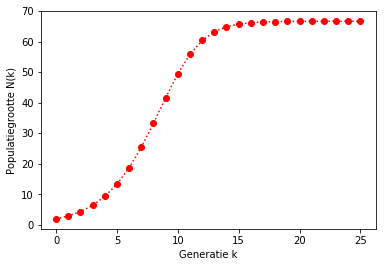
\includegraphics[width=8cm]{verhulst.png}\\
				\caption{Evolution of the population size $N$ as a function of the generation $k$.}
				\label{fig:verhulst}
			\end{figure}
			
			To what value does the number of individuals converge?
            $N$?
		\Question Discuss the influence of $N_0$ on the final number of individuals by repeating the calculations with $N_0 = 5$ and $N_0 = 25$.
		\Question Assume $K = 200$, $N_0 = 2$, $k = 25$, and let $r$ variate from 0.5 to 3.5 in steps of 0.5. Determine for each $r$ a plot of $N$ as a function of $K$. Describe what you see.
		\EndCurrentQuestion
\end{Exercise}

\begin{Answer}\phantom{}
    \Question If the function \texttt{verhulst} was used correctly, you get the vectors below $N$ and $T$.
        \begin{lstlisting}
>>> N
array([ 2.        ,  2.97      ,  4.38884325,  6.43880029,  9.34726431,
       13.36561134, 18.70862026, 25.43783685, 33.3036287 , 41.63695542,
       49.4531627 , 55.8376293 , 60.3726376 , 63.22254112, 64.85563889,
       65.73655412, 66.19512207, 66.42922671, 66.54752386, 66.6069888 ,
       66.63680102, 66.65172715, 66.65919524, 66.66293053, 66.6647985 ,
       66.66573255])

>>> T
array([ 0,  1,  2,  3,  4,  5,  6,  7,  8,  9, 10, 11, 12, 13, 14, 15, 16,
       17, 18, 19, 20, 21, 22, 23, 24, 25])
        \end{lstlisting}	
	\Question The number of individuals $N$ converges to about 67.
	\Question $N0$ has \textbf{no} influence on the final number of individuals.
	\Question If $r = 0.5$ the population becomes extinct. If $r$ increases, the final number of individuals increases. From $r = 2.5$, the gradient shows oscillations that increase as $r$ increases. With $r = 3.0$ and $r = 3.5$ it is therefore not clear how large the final number of individuals will be. Figure
    \ref{fig:verhulstR} summarises this.
	\EndCurrentQuestion
\end{Answer}

%oefening 2.7
\begin{Exercise}Consider the Verhulst model from the previous exercise. Suppose the individuals are harvested at a rate
 $h$ [T$^{-1}$] and the number of individuals harvested is proportional to the number of individuals:

	$$
	N_{k+1} = r\left(1 - \frac{N_k}{K}\right)N_k - h\,N_k\,.
	$$
    Assume $h = 0.125$ s$^{-1}$.
    \Question Write a function \texttt{verhulst2} with inputs $r$, $K$, $N0$, and $k$ and which calculates the number of individuals $N_k$ after each generation. The outputs of your function are a vector $N$ with $k+1$ elements ($N0$ as the first element), and a vector $T$. The latter contains the numbers $0$ to $k$.

    \Question Assume $r = 1.5$, $K = 200$, $N_0 = 2$, $k = 25$, and calculate the population size $N_k$ after each generation.
    \Question Make a figure in which you plot $N$ as a function of $T$. You should get Figure ~\ref{fig:verhulst2}.
    \begin{figure}[H]
				\centering
				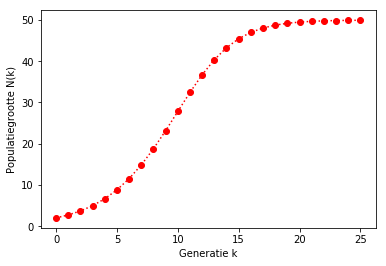
\includegraphics[width=8cm]{verhulst2.png}\\
				\caption{Evolution of the population size $N$ as a function of the generation $k$.\label{fig:verhulst2}}
	\end{figure}
	To what value does the number of individuals $N$ converge?		
    \Question Discuss the influence of the parameter $h$ on the final number of individuals by repeating the calculations with $h = 0.25$ s$^{-1}$ and $h = 0.75$ s$^{-1}$.
    \Question Assume $K = 200$, $N_0 = 2$, $k = 25$,and let $r$ vary from 0.5 to 3.5 in 0.5 increments. For each $r$, make a plot of $N$ as a function of $K$. Describe what you see.
    \EndCurrentQuestion
\end{Exercise}

\begin{Answer}\phantom{}
    \Question THe function \texttt{verhulst2} is a simple extension of the function \texttt{verhulst}.
    \Question If the function was written correctly, you get the following vectors $N$ and $T$.
\begin{lstlisting}
>>> N 
array([ 2.        ,  2.72      ,  3.684512  ,  4.96438678,  6.64119331,
        8.80084993, 11.52025646, 14.84498032, 18.75904713, 23.15442594,
       27.81637986, 32.4443899 , 36.71624784, 40.37421936, 43.28896971,
       45.46782161, 47.0133337 , 48.06643224, 48.76348002, 49.21570765,
       49.50520392, 49.68891628, 49.80484688, 49.87774366, 49.92347769,
       49.95212964])

>>> T
array([ 0,  1,  2,  3,  4,  5,  6,  7,  8,  9, 10, 11, 12, 13, 14, 15, 16,
       17, 18, 19, 20, 21, 22, 23, 24, 25])
\end{lstlisting}
    \Question The number of individuals
    $N$ converges to about 50.
    \Question If $h = 0.25$ the final number of individuals drops to about 32. If $h = 0.75$ the population dies out over time.
    \Question The observations are similar to those from the previous assignment. Figure \ref{fig:verhulstR} summarises this.
\begin{figure}[H]
				\centering
				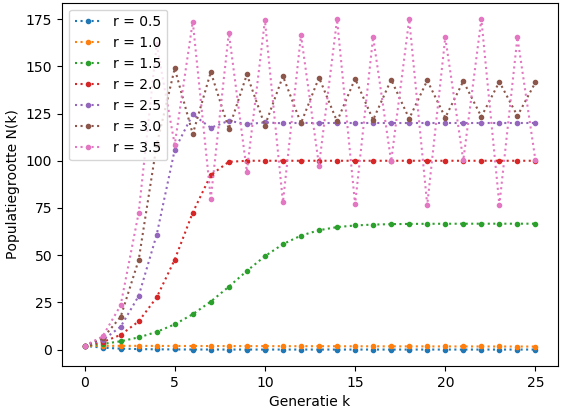
\includegraphics[width=10cm]{verhulstR.png}\\
				\caption{Evolution of the population size $N$ as a function of $r$.\label{fig:verhulstR}}
			\end{figure}
\begin{figure}[H]
				\centering
				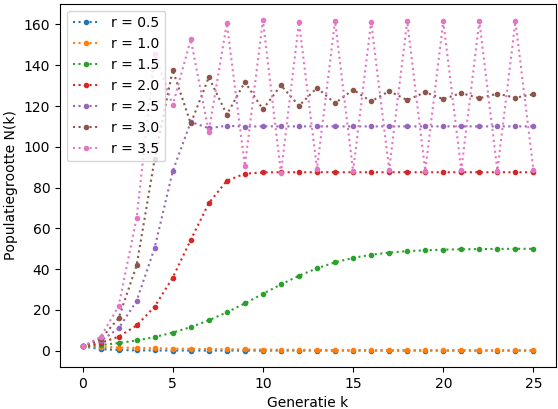
\includegraphics[width=10cm]{verhulstR2.png}\\
				\caption{Evolution of the population size $N$ as a function of $r$.\label{fig:verhulstR}}
			\end{figure}
 \EndCurrentQuestion
\end{Answer}    

%%%%%%%%%%%%%%%%%%%%%%%%%%%%
%Oude oefeningen nederlands, zonder oefeningenomgeving
%%%%%%%%%%%%%%%%%%%%%%%%%%%%

% \newpage
% \section{Exercises}
% \begin{enumerate}
% \item Determine the order and degree of the following differential equations.
% \begin{enumerate}
% \item $dy + \left(ty-\cos(t)\right)\, dt=0$
% \item $\left(y'''\right)^2+ty''+2y\left(y'\right)^3+ty=0$
% \item $y''\,y'+t\,y'^3+y=0$
% \item $y'+t=\left(y-ty'\right)^{-3}$
% \end{enumerate}

% \item Show that following families of curves can be written with one constant.
% \begin{enumerate}
%     %\item $y=t^2+C_1+C_2$
%     \item $y=C_1\, e^{t+C_2}$
%     \item $y=C_1+\ln |C_2 t|$
% \end{enumerate}

% \item Show that the function $y(t)$ is a solution of the given differential equation. Then, find the particular solution based on the initial conditions.
% \par
% \setlength{\arraycolsep}{0.28cm} 
% $\begin{array}{r|l|l|l}
% &\mbox{Differential equation} & \mbox{Solution} & \mbox{Initial condition(s)}\\ 
% \hline
% \hline
% &&&\vspace{-0.3cm}\\
% \hspace{-0.2cm}\mbox{(a)} &  y + y' = t^3 + 3 t^2\quad\; & y(t) = t^3 + Ce^{-t} &  y(0)=3 \\
% \hspace{-0.2cm}\mbox{(b)} &  t y' - y = t^2 e^t & y(t) = Ct + t e^{t} &  y(1)=e \\
% %\hspace{-0.2cm}\mbox{(c)} &  2 y - 3 t + t y'= 0 & y(t) = t + \dfrac{C}{t^2} &  y(-3)=-2 \\
% \hspace{-0.2cm}\mbox{(c)} &  y - t y' - y'{^2} = 0 & y(t) = C t + C^2 &  y(2)=-1 \\
% %\hspace{-0.2cm}\mbox{(e)} &  2 y - 2 t y' + t^2 y'' = 0 & y(t) = C_1 t + C_2 t^2 &  y(1)=0; y'(1)=5 \\
% \hspace{-0.2cm}\mbox{(d)} &  y''' + y'' = 0 & y(t) = C_1 e^{-t} + C_2 t + C_3\quad\; &  y(0)=2,\, y'(0)= 1,\, y''(0)= 3\\
% %\hspace{-0.2cm}\mbox{(g)} &  ty' + y = t\sin t & y(t) = \dfrac{\sin t+C}{t}-\cos t  &  y(\pi)=1 \\
% \hspace{-0.2cm}\mbox{(e)} &  y' - y = 2(1-t) & y(t) = 2t+Ce^t  &  y(0)=3 \\ %ADB
% %\hspace{-0.2cm}\mbox{(f)} &   y'' -3 y'+2y=2t-3 = 0 & y(t) = C_1 e^{t} + C_2 e^{2t} + t &  y(0)=0; y'(0)=2 \\ %ADB
% %\hspace{-0.2cm}\mbox{(g)} &  y'' + y = 0 & y(t) = C_1 \cos t + C_2 \sin t  &  y(0)=0; y'(0)=1 %ADB
% \end{array}$

% \item Construct the differential equations that describe the problems below.
% \begin{enumerate}
% %\item A puppy gains weight, $W$, at a rate approximately inversely proportional to its age, $t$, in months. % W' = k/t
% \item It has been empirically established that the rate at which the stomach volume V of a predatory fish decreases is directly proportional to the square root of this volume.
% \item During a chemical reaction, substance $A$ is converted to substance $B$ at a rate that is directly proportional to the square of the amount of substance $A$. Call $A(t)$ the amount of unreacted substance $A$ at time $t$.
% \item Newton's law of cooling states that the temperature change of an object is directly proportional to the difference between the (variable) temperature $T(t)$ of the object itself and the (constant) temperature $R$ of the environment.
% %\item[] The warming or cooling rate of a drink is proportional to the difference between the ambient temperature $T_a$ and the current temperature $T$ of the drink.
% \item When a patient is infused with a constant amount of painkiller per hour, the body breaks down this drug at a rate that is directly proportional to the amount present. We call that amount $M(t)$, the constant supply $a$ and the degradation rate $v$ (with $0< v < 1$), the relative amount of degraded substance per unit of time.
% %\item The fraction $P$ of the population who has heard a breaking news story increases at a rate proportional to the fraction of the population who has not yet heard the news story. % P' = k(1-P)
% %\item The fraction $A$ of reactants that have been converted increases at a rate proportional to the product of the fraction of converted reactants and the fraction of unconverted reactants. % A' = kA(1-A)
% %\item A radioactive material decays at a rate of change proportional to the current amount, $Q$, of the radioactive material. % Q' = -kQ
% % http://users.ugent.be/~jebossae/docs/differentiaalvergelijkingen.pdf
% % https://www.khanacademy.org/math/differential-equations/first-order-differential-equations/modal/e/write-differential-equations
% \end{enumerate}

% \ifmathematica
% \item Determine and plot the solution of the following differential equations using Mathematica.\fi
% \ifpython\item Determine and plot the solution of the following differential equations using Python.\fi
% \begin{enumerate}
%     \item $y'=1+2ty$,\qquad if\quad $y(2)=-1$ %BDB
%     \item $y'+2ty=4t$,\qquad if\quad $y(0)=5$ %BDB
%     \item $(2+\sin (y))y'+t=0$,\qquad if\quad $y(2)=0$ %BDB
%     \item $x^2\,y\,y'-e^y=0$,\qquad if\quad $y\left(1\right)=0$ %BDB-P1
%     \item $y'' + 2y'+5y=0$,\qquad if\quad $y(0)=2$\quad and\quad $y'(0)=2$ %BDB
%     \item $ty'' + \left(\cos(t)\right)y'+t^2y=t$,\qquad if\quad $y(-1)=-1$\quad and\quad $y'(-1)=2$ %BDB
%     \item $y^{(4)}-4y'''-5y''+36y'-36\,y=0$,\qquad if\quad $y(0)=1,~y'(0)=2,~y''(0)=3$ and $y'''(0)=4$ %BDB-P1
% \end{enumerate}

% 	\item Consider Verhulst's logistic population model (Equation \eqref{verhulst}, Section 1.1.2):
% 	$$
% 	N_{k+1} = r\left(1 - \frac{N_k}{K}\right)N_k\,,
% 	$$
% with $r$ the growth factor $\left[-\right]$, $K$ the carrying capacity of the environment $\left[-\right]$, and $k$ $\left[-\right]$ the number of generations. $N_0$ $\left[-\right]$ represents the initial number of individuals.
% 		\begin{enumerate}
% 			\item Write a function \texttt{disguised} that takes $r$, $K$, $N0$, and $k$ as inputs and calculates the number of individuals $N_k$ after each generation. The outputs of your function are a vector $N$ with $k+1$ elements ($N0$ as the first element), and a vector $T$. The latter contains the numbers $0$ to $k$.
% 			\item Let $r = 1.5$, $K = 200$, $N_0 = 2$, $k = 25$, and calculate the population size $N_k$ after each generation.
% 			\item Make a figure in which you plot $N$ as a function of $T$. You should obtain Figure~\ref{fig:verhulst}.
			
% 			\begin{figure}[ht]
% 				\centering
% 				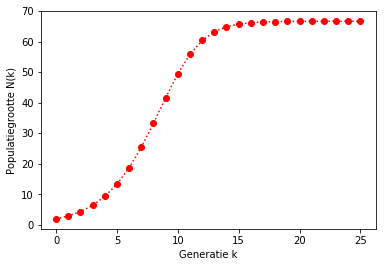
\includegraphics[width=8cm]{verhulst.png}\\
% 				\caption{Evolution of the population size $N$ as a function of the generation $k$.\label{fig:verhulst}}
% 			\end{figure}
			
% 			To what value does the number of individuals $N$ converge?
% 			\item Discuss the influence of $N_0$ on the final number of individuals by repeating the calculations with $N_0 = 5$ and $N_0 = 25$.
% 			%\item Set $N_0 = 5$ and repeat the calculations (other parameters the same). To what value does the number of individuals $N$ converge now? 
% 			%\itemSet $N_0 = 25$ and repeat the calculations (other parameters the same). To what value does the number of individuals $N$ converge now? Does the choice of $N_0$ have an influence?
% 			\item Set $K = 200$, $N_0 = 2$, $k = 25$, and let $r$ vary from 0.5 to 3.5 in increments of 0.5. For each $r$, plot $N$ as a function of $K$. Describe what you see.
% 		\end{enumerate}

% \item Consider the Verhulst model from the previous exercise. Suppose the individuals are harvested at a rate $h$ [T$^{-1}$] and the number of individuals harvested is proportional to the number of individuals:
% 	$$
% 	N_{k+1} = r\left(1 - \frac{N_k}{K}\right)N_k - h\,N_k\,.
% 	$$
% Let $h = 0.125$ s$^{-1}$.
% 		\begin{enumerate}
% 			\item Write a function \texttt{verhulst2} that takes $r$, $K$, $N0$, and $k$ as inputs and calculates the number of individuals $N_k$ after each generation. The outputs of your function are a vector $N$ with $k+1$ elements ($N0$ as the first element), and a vector $T$. The latter contains the numbers $0$ to $k$.
% 			\item Set $r = 1.5$, $K = 200$, $N_0 = 2$, $k = 25$, and calculate the population size $N_k$ after each generation.
% 			\item Make a figure in which you plot $N$ as a function of $T$. You should obtain Figure~\ref{fig:verhulst2}.
			
% 			\begin{figure}[ht]
% 				\centering
% 				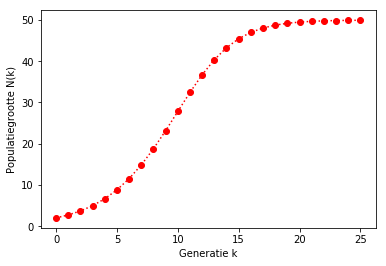
\includegraphics[width=8cm]{verhulst2.png}\\
% 				\caption{Evolution of the population size $N$ as a function of the generation $k$.\label{fig:verhulst2}}
% 			\end{figure}
			
% 			To what value does the number of individuals $N$ converge?
% 			\item Discuss the influence of the parameter $h$ on the final number of individuals by repeating the calculations with $h = 0.25$ s$^{-1}$ and $h = 0.75$ s$^{-1}$.
% 			%\item Set $N_0 = 5$ and repeat the calculations (other parameters the same). To what value does the number of individuals $N$ converge now?
% 			%\item Set $N_0 = 25$ and repeat the calculations (other parameters the same). To what value does the number of individuals $N$ converge now? Does the choice of $N_0$ have an influence?
% 			\item Set $K = 200$, $N_0 = 2$, $k = 25$, and let $r$ vary from 0.5 to 3.5 in increments of 0.5. For each $r$, plot $N$ as a function of $K$. Describe what you see.
% 		\end{enumerate}
% \end{enumerate}